\documentclass[10pt,letterpaper]{article} 
%\usepackage{tikz}
\usepackage{amsmath,amssymb,geometry,caption,subcaption}
%\usepackage{graphicx}‎‎
%\usefonttheme{serif}‎
%\usepackage{ptext}‎
\usepackage{xepersian}
%\settextfont{B Nazanin}
\usepackage{lipsum}
\setlength{\parindent}{0pt}
%\usepackage{enumitem}
%\setlist[enumerate,1]{label=(\arabic*)}
\newcommand{\pf}{$\blacksquare$}
\newcommand{\EX}{\Bbb E}
\newcommand{\nl}{\newline\newline}
\setlength{\parskip}{1em}

\usepackage{amsmath}
\usepackage{accents}
\newlength{\dhatheight}
\newcommand{\doublehat}[1]{%
    \settoheight{\dhatheight}{\ensuremath{\hat{#1}}}%
    \addtolength{\dhatheight}{-0.35ex}%
    \hat{\vphantom{\rule{1pt}{\dhatheight}}%
    \smash{\hat{#1}}}}

\newcounter{QuestionNumber}
\setcounter{QuestionNumber}{1}

\newcommand{\Q}{
\textbf{
سوال \theQuestionNumber)
}
\stepcounter{QuestionNumber}
}

\newcommand{\fig}[3]{
\begin{figure}[h!]
#1
\caption{#2}
\label{#3}
\end{figure}
}

\newcommand{\subfig}[3]{
\begin{subfigure}{#3}
#1
\caption{#2}
\end{subfigure}
}

\newcommand{\qn}[1]{
\[
\begin{split}
#1
\end{split}
\]
}
%\newcommand{\pic}[2]{
%\begin{center}
%\includegraphics[width=#2]{#1}
%\end{center}
%}
\begin{document}
\Large
\begin{center}
به نام زیبایی

پاسخ تمرینات سری یازدهم سیگنال ها و سیستم ها

\hrulefill
\end{center}
%\Q
%
%تبدیل فوریه‌ی سیگنال های زمان گسسته‌ی زیر را به دست آورید.
%
%الف)
%$
%x[n]=u[n]-u[n-5]
%$
%
%ب)
%$
%x[n]=({1\over 3})^nu[n]
%$
%
%پ)
%$
%x[n]=-({1\over 3})^nu[-n-1]
%$
%
%ت)
%$
%x[n]=\sin{\pi\over 2}n+\cos n
%$
%
%ث) 
%$
%x[n]=n({1\over 3})^nu[n]
%$
%
%\Q
%
%عکس تبدیل فوریه‌ی سیگنال های زیر را به دست آورید.
%
%الف)
%$
%X(e^{j\omega})=\sum_{k=-\infty}^{\infty}(-1)^k\delta(\omega-{\pi\over 2}k)
%$
%
%ب)
%$
%X(e^{j\omega})={1-{1\over 3}e^{-j\omega}\over 1-{1\over 4}e^{-j\omega}-{1\over 8}e^{-2j\omega}}
%$
%
%پ) 
%$
%X(e^{j\omega})={1\over 1-e^{-4j\omega}}
%$

\large

\Q

الف)
\qn{
x[n]&=(-\frac{1}{2})^n\sin 2nu[n]
=(-\frac{1}{2})^n\frac{e^{2jn}-e^{-2jn}}{2j}u[n]
\\&\iff
\frac{1}{2j}\left[\frac{1}{1+\frac{1}{2}e^{2jn}z^{-1}}-\frac{1}{1+\frac{1}{2}e^{-2jn}z^{-1}}\right]
}
$$
ROC=\{|z|>\frac{1}{2}\}
$$

ب) برای این سیگنال داریم
\qn{
X(z)&=\sum_{n=-\infty}^\infty \frac{1}{n\cdot 2^n}z^{-n}
\\&=\sum_{n=0}^\infty \frac{1}{n\cdot 2^n}z^{-n}
+
\sum_{n=-\infty}^{-1} \frac{1}{n\cdot 2^n}z^{-n}
}
از آنجایی که سری اول در 
$
|z|>\frac{1}{2}
$
و سری دوم در 
$
|z|<\frac{1}{2}
$
همگرا می شود و این دو ناحیه همگرایی اشتراک ندارند، در نتیجه این سیگنال تبدیل z ندارد.

پ) طبق تعریف:
\qn{
X(z)&=\sum_n \left[(-1)^nu[n]+\alpha^n u[-n-1]\right]z^{-n}
\\&=\sum_n \left[(-1)^nu[n]+\sum_n \alpha^n u[-n-1]\right]z^{-n}
\\&=\sum_n (-1)^nu[n]z^{-n}+\sum_n \alpha^n u[-n-1]z^{-n}
\\&=\sum_{n=0}^\infty (-1)^nz^{-n}+\sum_{n=-\infty}^{-1} \alpha^n z^{-n}
\\&=\frac{1}{1+z^{-1}}-\frac{1}{1-\alpha z^{-1}}
}
که شرط وجود داشتن سری اول 
$
|z|>1
$
و شرط سری دوم 
$
|z|<|\alpha|
$
است؛ در نتیجه برای وجود داشتن تبدیل z باید داشته باشیم
$$
1<|\alpha|
$$
و در این صورت ناحیه همگرایی برابر 
$
1<|z|<|\alpha|
$
خواهد بود.

ت) تبدیل $z$ سیگنال 
$
(\frac{1}{2})^nu[n]
$
برابر
$
\frac{1}{1-\frac{1}{2}z^{-1}}
$
با ناحیه همگرایی
$
|z|>\frac{1}{2}
$
است؛ در نتیجه تبدیل z سیگنال 
$
x[n]
$
برابر
$$
X(z)=\frac{8z^3-\frac{1}{4z^2}}{1-\frac{1}{2}z^{-1}}
$$
با ناحیه همگرایی
$
|z|>\frac{1}{2}
$
است.

\Q

با تعریف 
$
u=z^{-1}
$
داریم:

الف) 
\qn{
X(z)&=\frac{1-\frac{1}{2}u}{(1-\frac{1}{3}u)(1+\frac{1}{4}u^2)}
\\&=\frac{1-\frac{1}{2}u}{(1-\frac{1}{3}u)(1+\frac{j}{2}u)(1-\frac{j}{2}u)}
\\&=\frac{-\frac{2}{13}}{1-\frac{1}{3}u}+\frac{\frac{15-3j}{26}}{1+\frac{j}{2}u}+\frac{\frac{15+3j}{26}}{1-\frac{j}{2}u}
\\&=\frac{-\frac{2}{13}}{1-\frac{1}{3}z^{-1}}+\frac{\frac{15-3j}{26}}{1+\frac{j}{2}z^{-1}}+\frac{\frac{15+3j}{26}}{1-\frac{j}{2}z^{-1}}
}

بنابراین
$$
x[n]=-\frac{2}{13}(\frac{1}{3})^nu[n]
-\frac{15+3j}{26}(\frac{j}{2})^nu[-n-1]
-\frac{15-3j}{26}(-\frac{j}{2})^nu[-n-1]
$$

ب)
\qn{
X(z)&=\frac{1}{(1-\frac{1}{2}z^{-1})(1-2z^{-1}+\frac{15}{16}z^{-2})}
\\&=\frac{1}{(1-\frac{1}{2}u)(1-2u+\frac{15}{16}u^2)}
\\&=\frac{1}{(1-\frac{1}{2}u)(1-\frac{4}{3}u)(1-\frac{4}{5}u)}
\\&=\frac{A}{1-\frac{1}{2}u}
+\frac{B}{1-\frac{4}{3}u}
+\frac{C}{1-\frac{4}{5}u}
\\&=\frac{1}{1-\frac{1}{2}u}
+\frac{4}{1-\frac{4}{3}u}
-\frac{4}{1-\frac{4}{5}u}
\\&=\frac{1}{1-\frac{1}{2}z^{-1}}
+\frac{4}{1-\frac{4}{3}z^{-1}}
-\frac{4}{1-\frac{4}{5}z^{-1}}
}
در نتیجه
$$
x[n]=4(\frac{4}{5})^nu[-n-1]-4(\frac{4}{3})^nu[-n-1]-(\frac{1}{2})^nu[-n-1]
$$

\Q

ناحیه همگرایی $H(z)$ شامل دایره واحد می شود در نتیجه 
$
ROC=\{\frac{1}{2}<|z|<2\}
$.
تبدیل z سیگنال $x[n]$ برابر است با
\qn{
&
X(z)=\frac{1}{1-\frac{1}{3}z^{-1}}+\frac{1}{1+\frac{1}{3}z^{-1}}
=
\frac{2}{(1-\frac{1}{3}z^{-1})(1+\frac{1}{3}z^{-1})}
\\&
ROC=\{|z|>\frac{1}{3}\}
}
بنابراین
$$
Y(z)=X(z)H(z)
=\frac{2}{(1-\frac{1}{2}z^{-1})(1+\frac{1}{3}z^{-1})(1-2z^{-1})^2}
$$
که دارای ناحیه همگرایی 
$
ROC=\{\frac{1}{2}<|z|<2\}
$
است. با تجزیه به کسرهای جزئی خواهیم داشت:
$$
Y(z)=
\frac{\frac{2}{15}}{1-\frac{1}{2}z^{-1}}
+
\frac{\frac{4}{245}}{1+\frac{1}{3}z^{-1}}
-
\frac{\frac{64}{147}}{1-2z^{-1}}
+
\frac{\frac{16}{7}}{(1-2z^{-1})^2}
$$
و در نتیجه
$$
y[n]=
\frac{2}{15}(\frac{1}{2})^nu[n]
+
\frac{4}{245}(-\frac{1}{3})^nu[n]
+
\frac{64}{147}(2)^nu[-n-1]
+\frac{8}{7}(n+1)2^nu[-n-2]
$$

\Q

الف) چون سیستم 1 پایدار است، در نتیجه ناحیه همگرایی آن به صورت 
$
0.8<|z|<1.2
$
 خواهد بود؛ در نتیجه این سیستم غیرعلی و دوطرفه است.

ب) سیستم 2 علی است؛ پس ناحیه همگرایی آن 
$
|z|>1
$
 بوده که شامل دایره واحد نمی شود؛ در نتیجه سیستم ناپایدار است.

پ) تنها صفر وافع در $-1$ از $X(z)$، روی دایره واحد افتاده و صفری از 
$
X(e^{j\omega})
$
 نیز هست؛ پس 
$
X(e^{j\omega})
$
 تنها در 
$
\omega=\pi
$
 صفر می شود (همجنین مضارب فرد $\pi$ به دلیل متناوب بودن $X(e^{j\omega})$).

ت) در سیستم معکوس، جای صفر و قطب های سیستم اصلی عوض می شوند؛ بنابراین نمودار صفر-قطب سیستم معکوس به صورت زیر است:
\vspace{0.15cm}
\begin{figure}[h!]
\centering
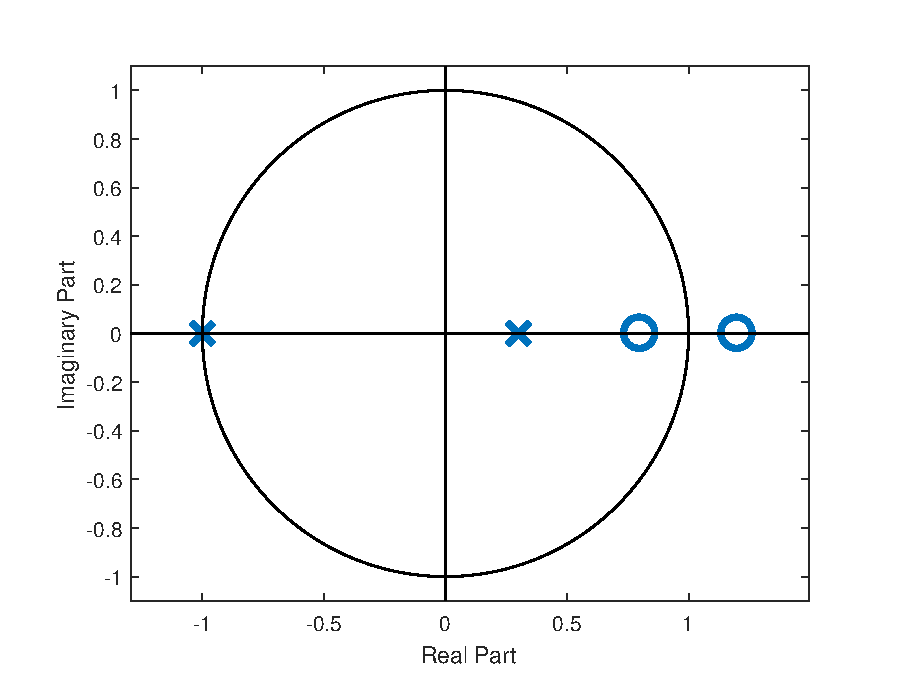
\includegraphics[width=100mm]{PSol12_Q3.eps}
\end{figure}

از طرفی باید ناحیه همگرایی سیستم معکوس، با ناحیه همگرایی سیستم اصلی اشتراک داشته باشد. سه ناحیه همگرایی ممکن برای سیستم معکوس عبارتند از:
\qn{
&(1) : |z|<0.3
\\&(2) : 0.3<|z|<1
\\&(3) : |z|>1
}{}
که از این بین، فقط نواحی 2 و 3 دارای اشتراک با 
$
0.8<|z|<1.2
$
هستند که نتیجه می شود سیستم اصلی دو معکوس دارد (این امر تناقضی محسوب نمی شود؛ زیرا دو معکوس ماهیتا متفاوتند؛ یکی ناپایدار و علی و دیگری ناپایدار و غیرعلی است).

ث) شکل پاسخ فرکانسی سیستم 1، به شکل بالاست؛ بنابراین، این سیستم یک فیلتر پایین گذر است.
\vspace{.1cm}
\begin{figure}[h!]
\centering
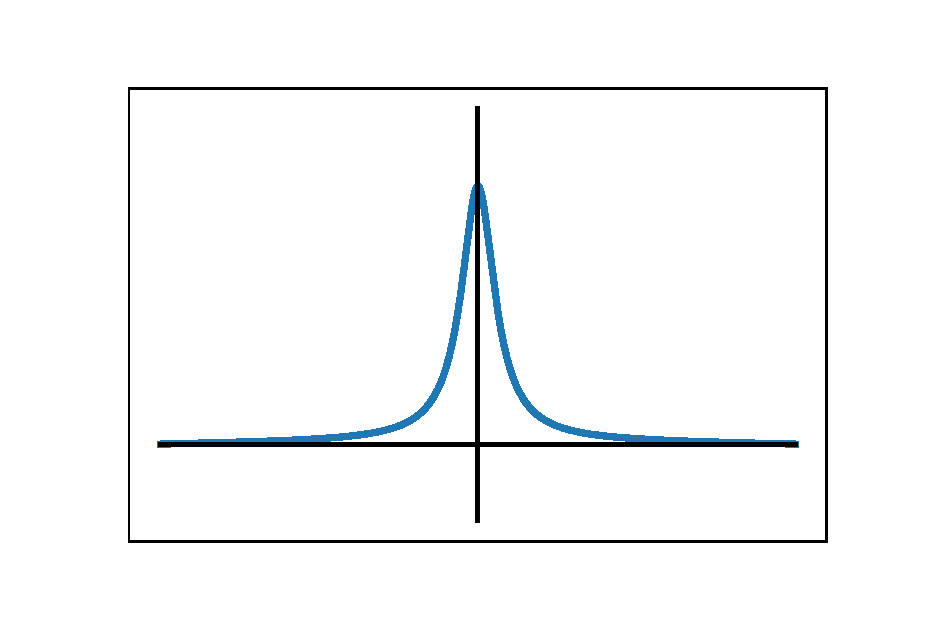
\includegraphics[width=100mm]{PSol12_Q3_5.eps}
\end{figure}
\vspace{.1cm}


\Q

\qn{
H(z)&=A\frac{z}{(z+\frac{1}{2})(z-\frac{3}{2}e^{j\frac{\pi}{4}})(z-\frac{3}{2}e^{-j\frac{\pi}{4}})}
\\&=
A\frac{z^{-2}}{(1+\frac{1}{2}z^{-1})(1-\frac{3}{2}e^{j\frac{\pi}{4}}z^{-1})(1-\frac{3}{2}e^{-j\frac{\pi}{4}}z^{-1})}
}
از طرفی
\qn{
\frac{1}{(1+\frac{1}{2}z^{-1})(1-\frac{3}{2}e^{j\frac{\pi}{4}}z^{-1})(1-\frac{3}{2}e^{-j\frac{\pi}{4}}z^{-1})}
=
\frac{B}{1+\frac{1}{2}z^{-1}}
+
\frac{C}{1-\frac{3}{2}e^{j\frac{\pi}{4}}z^{-1}}
+
\frac{D}{1-\frac{3}{2}e^{-j\frac{\pi}{4}}z^{-1}}
}
که
\qn{
&
B=10+3\sqrt 2
\\&
C=\frac{1}{(1+j)(1+\frac{1}{3}e^{-j\frac{\pi}{4}})}
\\&
D=\frac{1}{(1-j)(1+\frac{1}{3}e^{j\frac{\pi}{4}})}
}
از طرفی می توان به دلخواه $A=1$ گرفت؛ زیرا در نوع پاسخ تاثیری ندارد.
$$
H(z)=
\frac{Bz^{-2}}{1+\frac{1}{2}z^{-1}}
+
\frac{Cz^{-2}}{1-\frac{3}{2}e^{j\frac{\pi}{4}}z^{-1}}
+
\frac{Dz^{-2}}{1-\frac{3}{2}e^{-j\frac{\pi}{4}}z^{-1}}
$$

الف) پایدار
$$
h[n]=
B(\frac{1}{2})^{n-2}u[n-2]
-
C(\frac{3}{2}e^{j\frac{\pi}{4}})^{n-2}u[-n+1]
-
D(\frac{3}{2}e^{-j\frac{\pi}{4}})^{n-2}u[-n+1]
$$
ب) علی و ناپایدار
$$
h[n]=
B(\frac{1}{2})^{n-2}u[n-2]
+
C(\frac{3}{2}e^{j\frac{\pi}{4}})^{n-2}u[n-2]
+
D(\frac{3}{2}e^{-j\frac{\pi}{4}})^{n-2}u[n-2]
$$
پ) ضدعلی
$$
h[n]=
-B(\frac{1}{2})^{n-2}u[-n+1]
-
C(\frac{3}{2}e^{j\frac{\pi}{4}})^{n-2}u[-n+1]
-
D(\frac{3}{2}e^{-j\frac{\pi}{4}})^{n-2}u[-n+1]
$$

\Q

سیستم حقیقی، زمان گسسته و پایدار $h[n]$ با تبدیل $z$ زیر توصیف می شود:
$$
H(z)={1-az^{-1}\over (1-2z^{-1})\left(1-{1\over 2}z^{-1}\right)}
$$

الف) اگر حذف صفر و قطب رخ ندهد، ناحیه همگرایی به صورت 
$
\frac{1}{2}<|z|<2
$
است و سیستم نمی تواند علی یا ضدعلی باشد. با این حال، اگر 
$
a=2
$
، سیستم علی و اگر 
$
a=\frac{1}{2}
$
سیستم ضدعلی خواهد بود.

ب) سیستم وارون به غیر از $z=0$ دارای حداکثر یک قطب در $z=a$ است؛ بنابراین برای علی و پایدار بودن باید داشته باشیم
$
|a|<1
$.
در این صورت، ناحیه همگرایی سیستم وارون به صورت
$
|z|>|a|
$
می باشد که همواره با 
$
\frac{1}{2}<|z|<2
$
،
$
\frac{1}{2}<|z|
$
و
$
|z|<2
$
اشتراک دارد؛ پس باید داشته باشیم
$
|a|<1
$
.
همچنین $a$ باید حقیقی باشد؛ زیرا وارون یک سیستم حقیقی، خود حقیقی است.

پ) نمودار صفر و قطب سیستم وارون در شکل 1 دیده می شود.
\begin{figure}[h!]
\centering
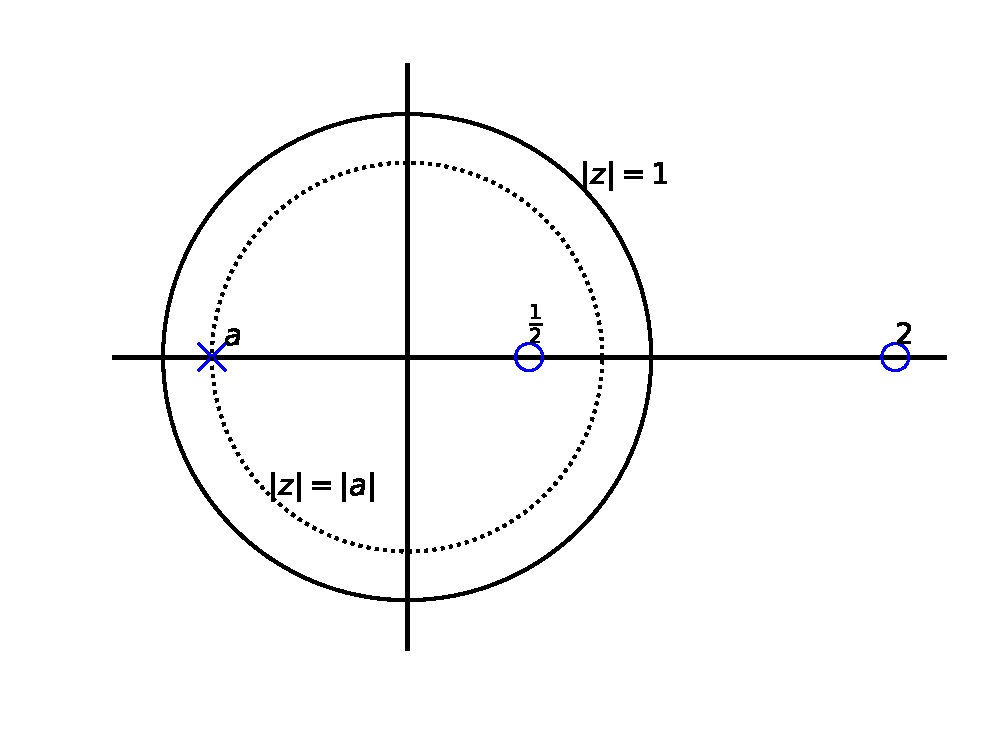
\includegraphics[width=100mm]{pz_inv.eps}
\caption{}
\end{figure}

\Q

از گزاره های 2 و 3 نتیجه می شود که $H(z)$ به صورت زیر است:
$$
H(z)=\frac{A(z-3)}{(z-2)(z-a)}
$$
با توجه به گزاره 4،
\qn{
&H(\frac{3}{2})=9\implies A+3a=\frac{9}{2}
\\&H(\frac{4}{3})=10\implies A+4a=\frac{16}{3}
}
در نتیجه
$$
a=\frac{5}{6}\quad,\quad A=2
$$
و
$$
H(z)=\frac{2(z-3)}{(z-2)(z-\frac{5}{6})}
$$

الف) نمودار صفر-قطب در شکل 2 مشخص است.

\begin{figure}[h!]
\centering
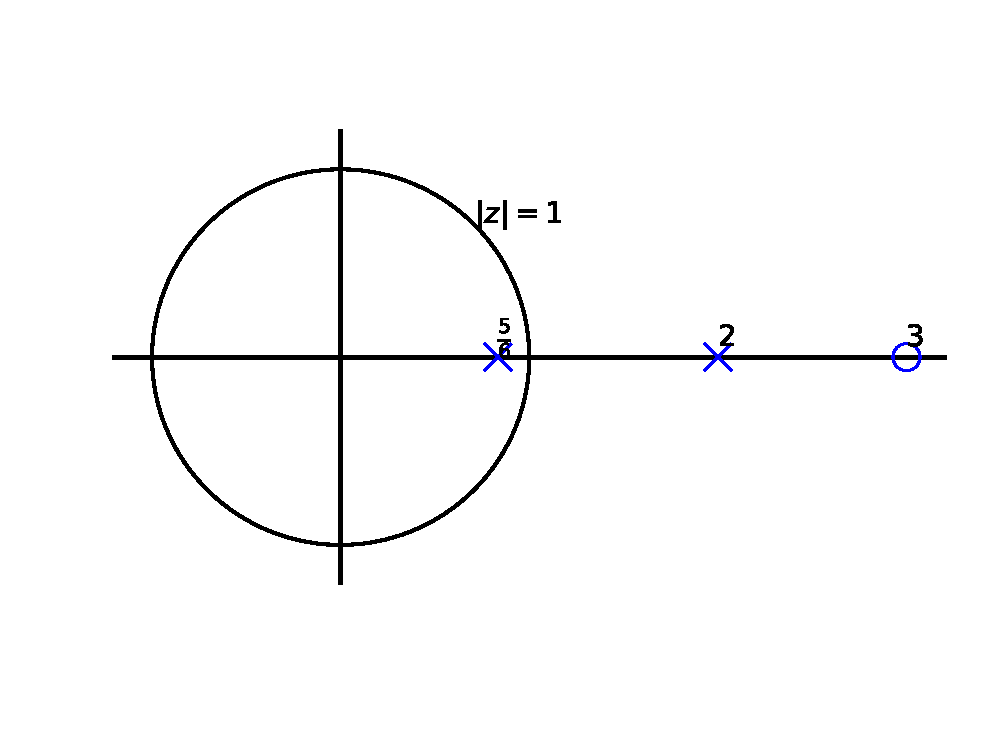
\includegraphics[width=110mm]{psol11_q7.eps}
\caption{}
\end{figure}

ب) پاسخ سیستم به ورودی 
$
x[n]=(-\frac{1}{4})^{n}
$
نامحدود است؛ زیرا 
$
z=-\frac{1}{4}
$
در ناحیه همگرایی سیستم وجود ندارد.

پ) 
$$
\hat H(z)=\frac{(z-2)(z-\frac{5}{6})}{2(z-3)}\quad,\quad |z|<3
$$
بنابراین
\qn{
\hat H(z)&=\frac{z}{2}+\frac{1}{12}+\frac{13}{12}\frac{1}{z-3}
\\&=\frac{z}{2}+\frac{1}{12}+\frac{13}{12}\frac{z^{-1}}{1-3z^{-1}}
}
و
$$
\hat h[n]=\frac{1}{2}\delta[n+1]+\frac{1}{12}\delta[n]-\frac{13}{36}\cdot 3^{n}u[-n]
$$
\end{document}